\documentclass[11pt, a4paper, twocolumn]{article}

\usepackage{fancyhdr} % Required for custom headers
\usepackage{extramarks} % Required for headers and footers
\usepackage{graphicx} % Required to insert images
\usepackage{courier} % Required for the courier font
\usepackage[utf8]{inputenc}
\usepackage{datetime}
\usepackage{amsmath}
\usepackage{amssymb}
\usepackage{arydshln}
\usepackage{mathtools}
\usepackage{caption}
\usepackage{float}
\usepackage{subcaption}
\usepackage{listings}
\usepackage{hyperref}
\usepackage{epstopdf}
\usepackage[left=1.75cm, right=1.75cm, bottom=3cm, top = 3cm]{geometry}
\usepackage{blindtext}
\usepackage{algorithm}				%För pseudokoder
\usepackage{algpseudocode}			%För pseudokoder
\usepackage{transparent}
%%\usepackage[table]{xcolor}% http://ctan.org/pkg/xcolor

%%%%%%%%%%%%%%%%%%%%%%% FOR DRAFT %%%%%%%%%%%%%%%%%%%%%%%%%%
\newcommand{\printdraft}{1} % If we want to print draft
%%% USAGE IN TEXT:
% 	\ifnum\printdraft>0
% 		OUR DRAFT TEXT GOES HERE
% 	\fi
%%%%%%%%%%%%%%%%%%%%%%% END DRAFT %%%%%%%%%%%%%%%%%%%%%%%%%%
\linespread{1.0} % Line spacing

% Set up the header and footer
%\pagestyle{fancy}
\lhead{J. Sahlström, A. Lindström \& D. Dürebrandt\\ \today} % Top left header
\rhead{Machine Learning Project} % Right center head
\chead{\firstxmark} % Center right header
\lfoot{\lastxmark} % Bottom left footer
\cfoot{\thepage} % Bottom center footer
%\rfoot{Page\ \thepage\ \protect\pageref{LastPage}} % Bottom right footer
\renewcommand\headrulewidth{0.4pt} % Size of the header rule
\renewcommand\footrulewidth{0.4pt} % Size of the footer rule
\newcommand\bigforall{\mbox{\LARGE $\mathsurround0pt\forall$}}  % Large for all symbol
\setlength{\columnsep}{30pt}
\setlength\parindent{0pt} % Removes all indentation from paragraphs

%----------------------------------------------------------------------------------------
%   TITLE PAGE
%----------------------------------------------------------------------------------------

\title{
%
\includegraphics[width=0.3\textwidth]{../img/uu-logo.pdf}\\
Machine Learning Project\\ \Large \emph{Classification of news articles}}
\author{
Jakob Sahlström \\ \scriptsize{jasa5691@student.uu.se} 
\and
Anders Lindström \\ \scriptsize{anli6945@student.uu.se} 
\and
Jesper Dürebrandt \\ \scriptsize{jedu6357@student.uu.se}
}
\date{Uppsala University\\\ \\\today} % Insert date here if you want it to appear below your name

%----------------------------------------------------------------------------------------

\usepackage{eso-pic}
\newcommand\BackgroundPic{%
\put(0,0){%
\parbox[b][1.66\paperheight]{\paperwidth}{%
\vfill
\centering
{\transparent{0.20}
\includegraphics[width=.8\paperwidth,height=.8\paperheight,trim=0 40 0 0, clip,%
keepaspectratio]{img/uu-logo.pdf}}%
\vfill
}}}

\begin{document}
\AddToShipoutPicture*{\BackgroundPic}
\twocolumn[
\begin{@twocolumnfalse}
\maketitle
\begin{abstract}
\blindtext
\end{abstract}
\end{@twocolumnfalse}
]
%\maketitle
%\thispagestyle{empty}
%\newpage
\setcounter{page}{1}
%\newpage
% \tableofcontents
% \newpage

\section{Introduction}
There are many different types of classifiers and they all have their advantages and disadvantages. In text classification, the samples typically have feature vectors of high dimensionality. This project investigates four classifiers that hypothetically work well for feature vectors of high dimensions, namely Bernoulli Na�ve Bayes, Mulitnomial Na�ve Bayes, Random Forest, and Support Vector Machine. 
\section{Theory}
Let $c$ be the class and $A = a_1, \dots ,a_n$ be the attributes of a document. Then with Bayes Theorem
\begin{equation}
p(c|A)=\frac{p(A|c)p(c)}{p(A)},
\end{equation}
the attributes $A$ is classified as class $C$ if and only if
\begin{equation}
f_b(A)=\frac{p(c|A)}{p(\neg c|A)} \geq 1,
\end{equation}
where $f_b(A)$ is called a $Bayesian$ classifier. Assuming all attributes are independent given the class, 
\[
p(A|c)=p(a_1,\dots ,a_n | c) = \prod_{i=1}^n p(a_i|c)
\]
the final classifier can be written as
\begin{equation}
f_{nb}(A) = \frac{p(c)}{p(\neg c)}\prod_{i=1}^n\frac{p(a_i|c)}{p(a_i|\neg c)}
\end{equation}
where $f_{nb}$ is called the \emph{Naive Bayesian} classifier.\\\\
Two models that uses the Naive Bayes assumption are the \emph{multi-variate Bernoulli} model and the \emph{multinomial} model. The main difference is that in the Bernoulli model the attributes are binary, indicating if a word from a vocabulary has occurred at least once or not. In the multinomial model the frequency of words are taken into account.
\subsection{Random Forest classifier}
Random Forest (RF) is based on building several considerably small decision trees. Consider having a feature vector that is of length $N$, then randomly select $n << N$ of those features. Build the trees with some kind of algorithm (e.g. C4.5), where information gain is taken into consideration when splitting, and no pruning is done (i.e. expand the tree fully). Then repeat selecting $n$ new variables from $N$ until the wanted number of trees are built.
\\\\
After all the trees are built, they can be used to let a new vector of data pass through all the trees and then letting each tree \emph{vote} on what class the vector most probably should be a part of.

\begin{algorithm}
\caption{Random Forest
    \label{alg:RF}}
\begin{algorithmic}
\State Let $x = (x_1,x_2,...,x_N)$ be a set of features;
\While {{\it not enough trees}}
	\State Randomly pick with replacement a subset containing $n << N$ features;
	\State Use training set to build a decision tree using a classification algorithm, e.g. C4.5, except no pruning is done.
\EndWhile
\end{algorithmic}
\end{algorithm}
\subsection{Support Vector Machine Classifier}
Support vector machine classifiers (SVM's) classifies data belonging to two classes by finding the hyperplane with the widest margin that separates the classes. The data vectors that restrict the margin of the hyperplane are referred to as support vectors. These also fully specify the decision function. Finding the optimal hyperplane is a maximization problem, where the objective function describes the width of the margin. The problem can be formulated using Lagrangian multipliers and is then solved using quadratic programming. An advantage with this approach is that the maximization problem is convex, meaning that the maximum found is guaranteed to be the global maximum. This requires, however, that the classes are linearly separable. If they are not, one can make use of a so called kernel function that maps the data onto a space in which the classes might be linearly separable. Support vector machines are suitable for problems with high dimensionality, but might perform badly if the number of samples is much smaller than the number of dimensions. \cite{Berwick03SVM}

\section{Method}
\subsection{Data retrieval}
A crawler was implemented to extract articles from BBC's RSS feed\footnote{\url{http://www.bbc.com/news/10628494}}. The crawler extracts the content of each article from eight different topics, namely
\begin{itemize}[noitemsep,nolistsep]
	\item Business
	\item Education
	\item Entertainment and Art
	\item Health
	\item Politics
	\item Science and Environment
	\item Sports
	\item Technology.
\end{itemize}
A total of 693 articles were extracted. As training set 2/3 of the articles were randomly selected and the remaining 1/3 were used as test set. Notable is that the distribution of topics is not uniform since the RSS feeds of the topics are not updated equally frequent. 
\subsection{Coding}
Python is chosen as programming language in order to extend our knowledge and experience of implementing different types of classifiers using the Scikit-learn machine learning library in python and further understand how the data has to be prepared and presented to the classifiers.
\subsection{Preparation of Data}
To classify the articles as accurately and fast as possible, the data is prepared in such way that it contains as much information as possible in a format as dense as possible. To achieve this, the articles are parsed into words with white-space as separator, then removed of all characters not found in the English alphabet, though keeping the '-' character. The words are stemmed so that similar words would be on the same form, and not be seen as two different words. (E.g. "argued", "argues", "arguing" are reduced to "argu".) After stemming, all so called stop words are removed (such as "a", "the", etc.). 
\subsection{Vocabulary}
The vocabulary is built up by unique stemmed words from the training set which consists of 66\% of all articles. By different pruning techniques the vocabulary is reduced in size and only the most informative elements are kept. For the feature selection the score is determined by the $\chi^2$ function. The vocabulary is then pruned by selecting a percentile of the best features.
\subsection{Datatypes}
There are many different ways to represent a feature vector, and different classifiers might want it represented in different ways. We have chosen to investigate a couple of different types of representations of the vocabulary. The different datatypes were
\begin{description}[noitemsep,nolistsep]
\item[Binary:]\ \\Does article contain word or not.
\item[Count:]\ \\How many times does article contain word.
\item[$L_2$-normalized:]\ \\ The count array normalized with the $L_2$ norm. 
\item[Mapped value from 0 to 1:]\ \\ $\frac{c_i}{\max(c)}$ where $c_i$ is the count of word $i$.
\end{description}

\subsection{Classifiers}
In the Scikit-learn package\footnote{\url{http://scikit-learn.org/}} there are plenty of different classifiers, amongst them the four we want to investigate. The four classifiers we will be investigating are
\begin{itemize}[noitemsep,nolistsep]
\item Naïve Bayes: Bernoulli
\item Naïve Bayes: Multinomial
\item Support Vector machines (SVM)
\item Random forest 
\end{itemize}
\section{Results}
Main focus of this report is to analyze, and compare between models, the performance impact of varying vocabulary size for different data types as well as difficulties of distinguishing the eight different topics. The result of the analysis can be seen in Figure \ref{fig:hitratio} \& \ref{fig:confmat} and Table \ref{tab:similarity}.\\\\
Figure \ref{fig:hitratio} shows, for the different models and data types, the overall hit ratio of correct classification as a function of vocabulary size after $\chi^2$ pruning. By comparing the figures it can be noted that the maximum accuracy of 76\% is attained with binary inputs by Multinomial at a vocabulary size of 1022 words. Another observation is that Bernoulli is sensitive to vocabulary size compared to other models and SVM seems in contrast to Bernoulli more robust to changes in vocabulary size. More results derived from these figures are that Random Forest is independent of the feature format and Hybrid follows the behavior of Multinomial.\\\\
The confusion matrices in Figure \ref{fig:confmat} describes the accuracy for specific topics. The rightmost column describes for a certain topic how many articles it contains and the accuracy of the topic. The bottom row describes for a certain predicted class, how many times that was the target class, and the accuracy when predicted. Analyzing the matrices one can observe that Sport and Education is fairly easy to classify in contrast to Technology and Education which is often misclassified as Science \& Environment and Business respectively. Notable is that Random Forest has a tendency of predicting Sports.\\\\
Figure \ref{fig:hitratio-data} shows, for each model, how the hit rate depends on number of articles used as training set.
In Table \ref{tab:similarity} a comparison of the similarity of prediction when mispredicting is shown. The values are resembles, given that both classifiers predicted wrong class, how many times they predicted the same class.
%Table of similarities
\begin{table}[h]\footnotesize
	\caption{Percentage that two classifiers, when both classifying wrong, classifies test to the same class. A total of 231 articles were tested. A vocabulary size of 511 words and the data type \emph{"Mapped value from 0 to 1"} was used.}
	\begin{tabular}{r|cccc}
	\ 		 	& Bernoulli & Multin. 	&RF 		&SVM \\ \hline
	Bernoulli 	&100\%   	&67.3\%   	&69.0\%   	&58.8\%\\
	Multin. 	&67.3\%  	&100\%   	&78.6\%   	&76.9\%\\
	RF 			&69.0\%   	&78.6\%  	&100\%   	&75.4\%\\
	SVM 		&58.8\%   	&76.9\%   	&75.4\%  	&100\%
	\end{tabular}
	\label{tab:similarity}
\end{table}
\onecolumn
\newcommand{\figwidth}{0.49\textwidth}
\begin{figure}[H]
	\centering
	\begin{subfigure}[b]{\figwidth}
		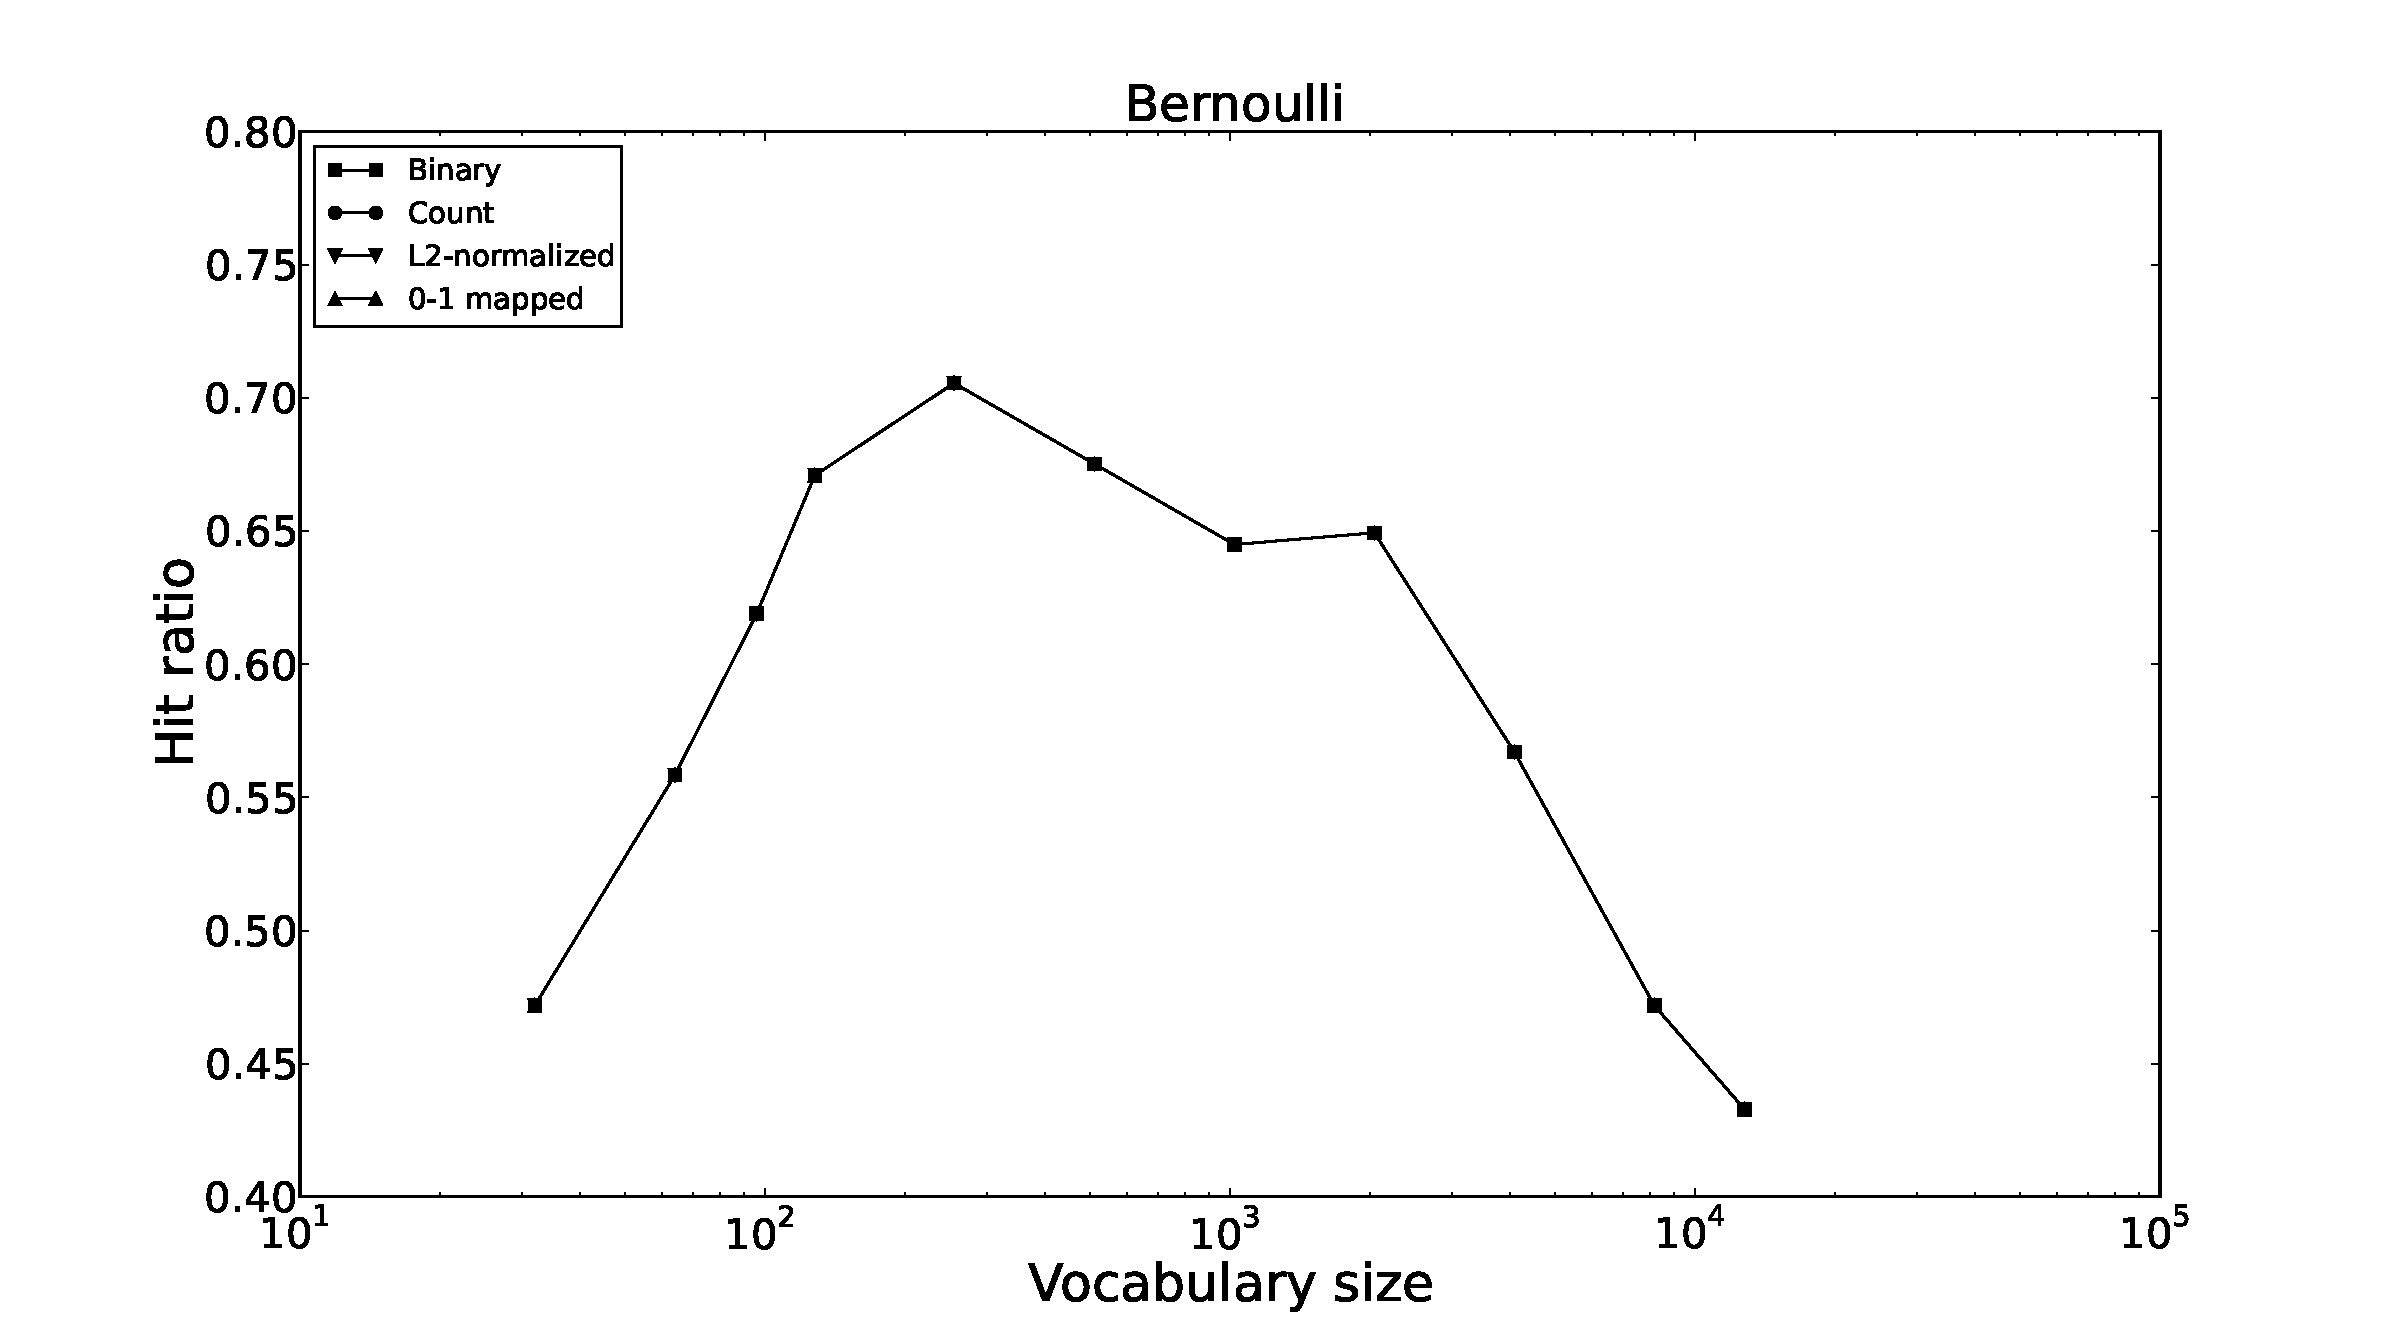
\includegraphics[width=\textwidth]{img/Bernoulli-hitrate-eps-converted-to.pdf}
		\caption{Hit ratio of Bernoulli classifier with varying vocabulary size. All values greater than zero is mapped to one, hence the different data types result in same accuracy.}
		\label{fig:hitratio-nb}
	\end{subfigure}
	~
	\begin{subfigure}[b]{\figwidth}
		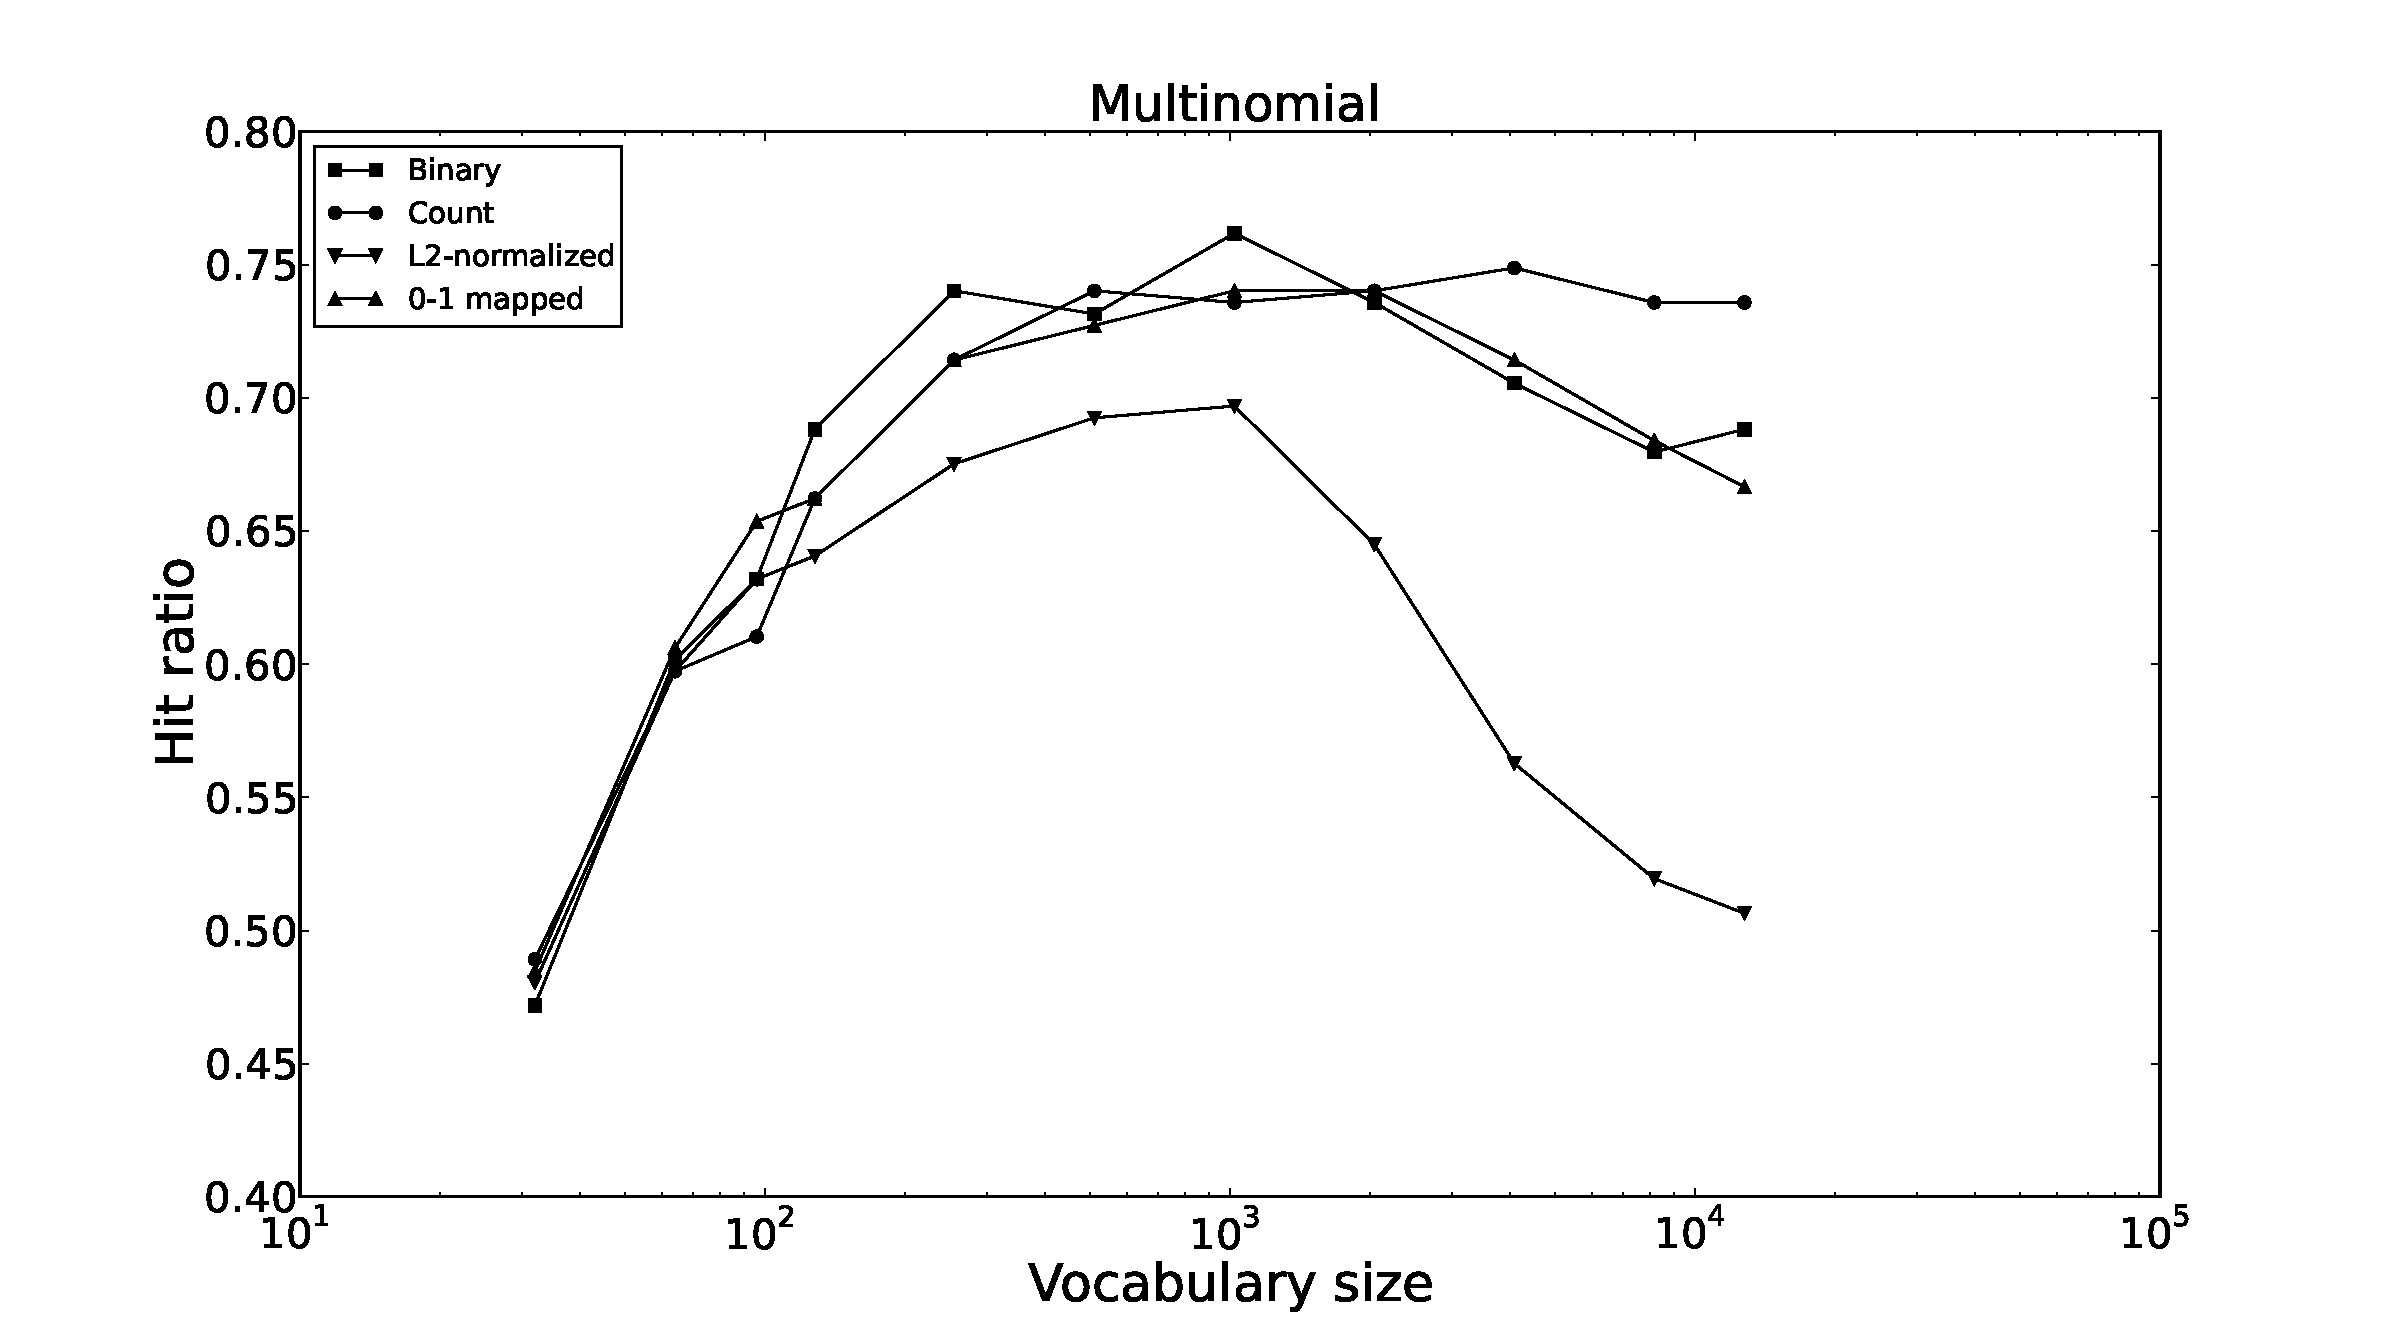
\includegraphics[width=\textwidth]{img/Multinomial-hitrate-eps-converted-to.pdf}
		\caption{Hit ratio of Multinomial classifier with varying vocabulary size.}
		\label{fig:hitratio-mn}
	\end{subfigure}
	\\
	\begin{subfigure}[b]{\figwidth}
		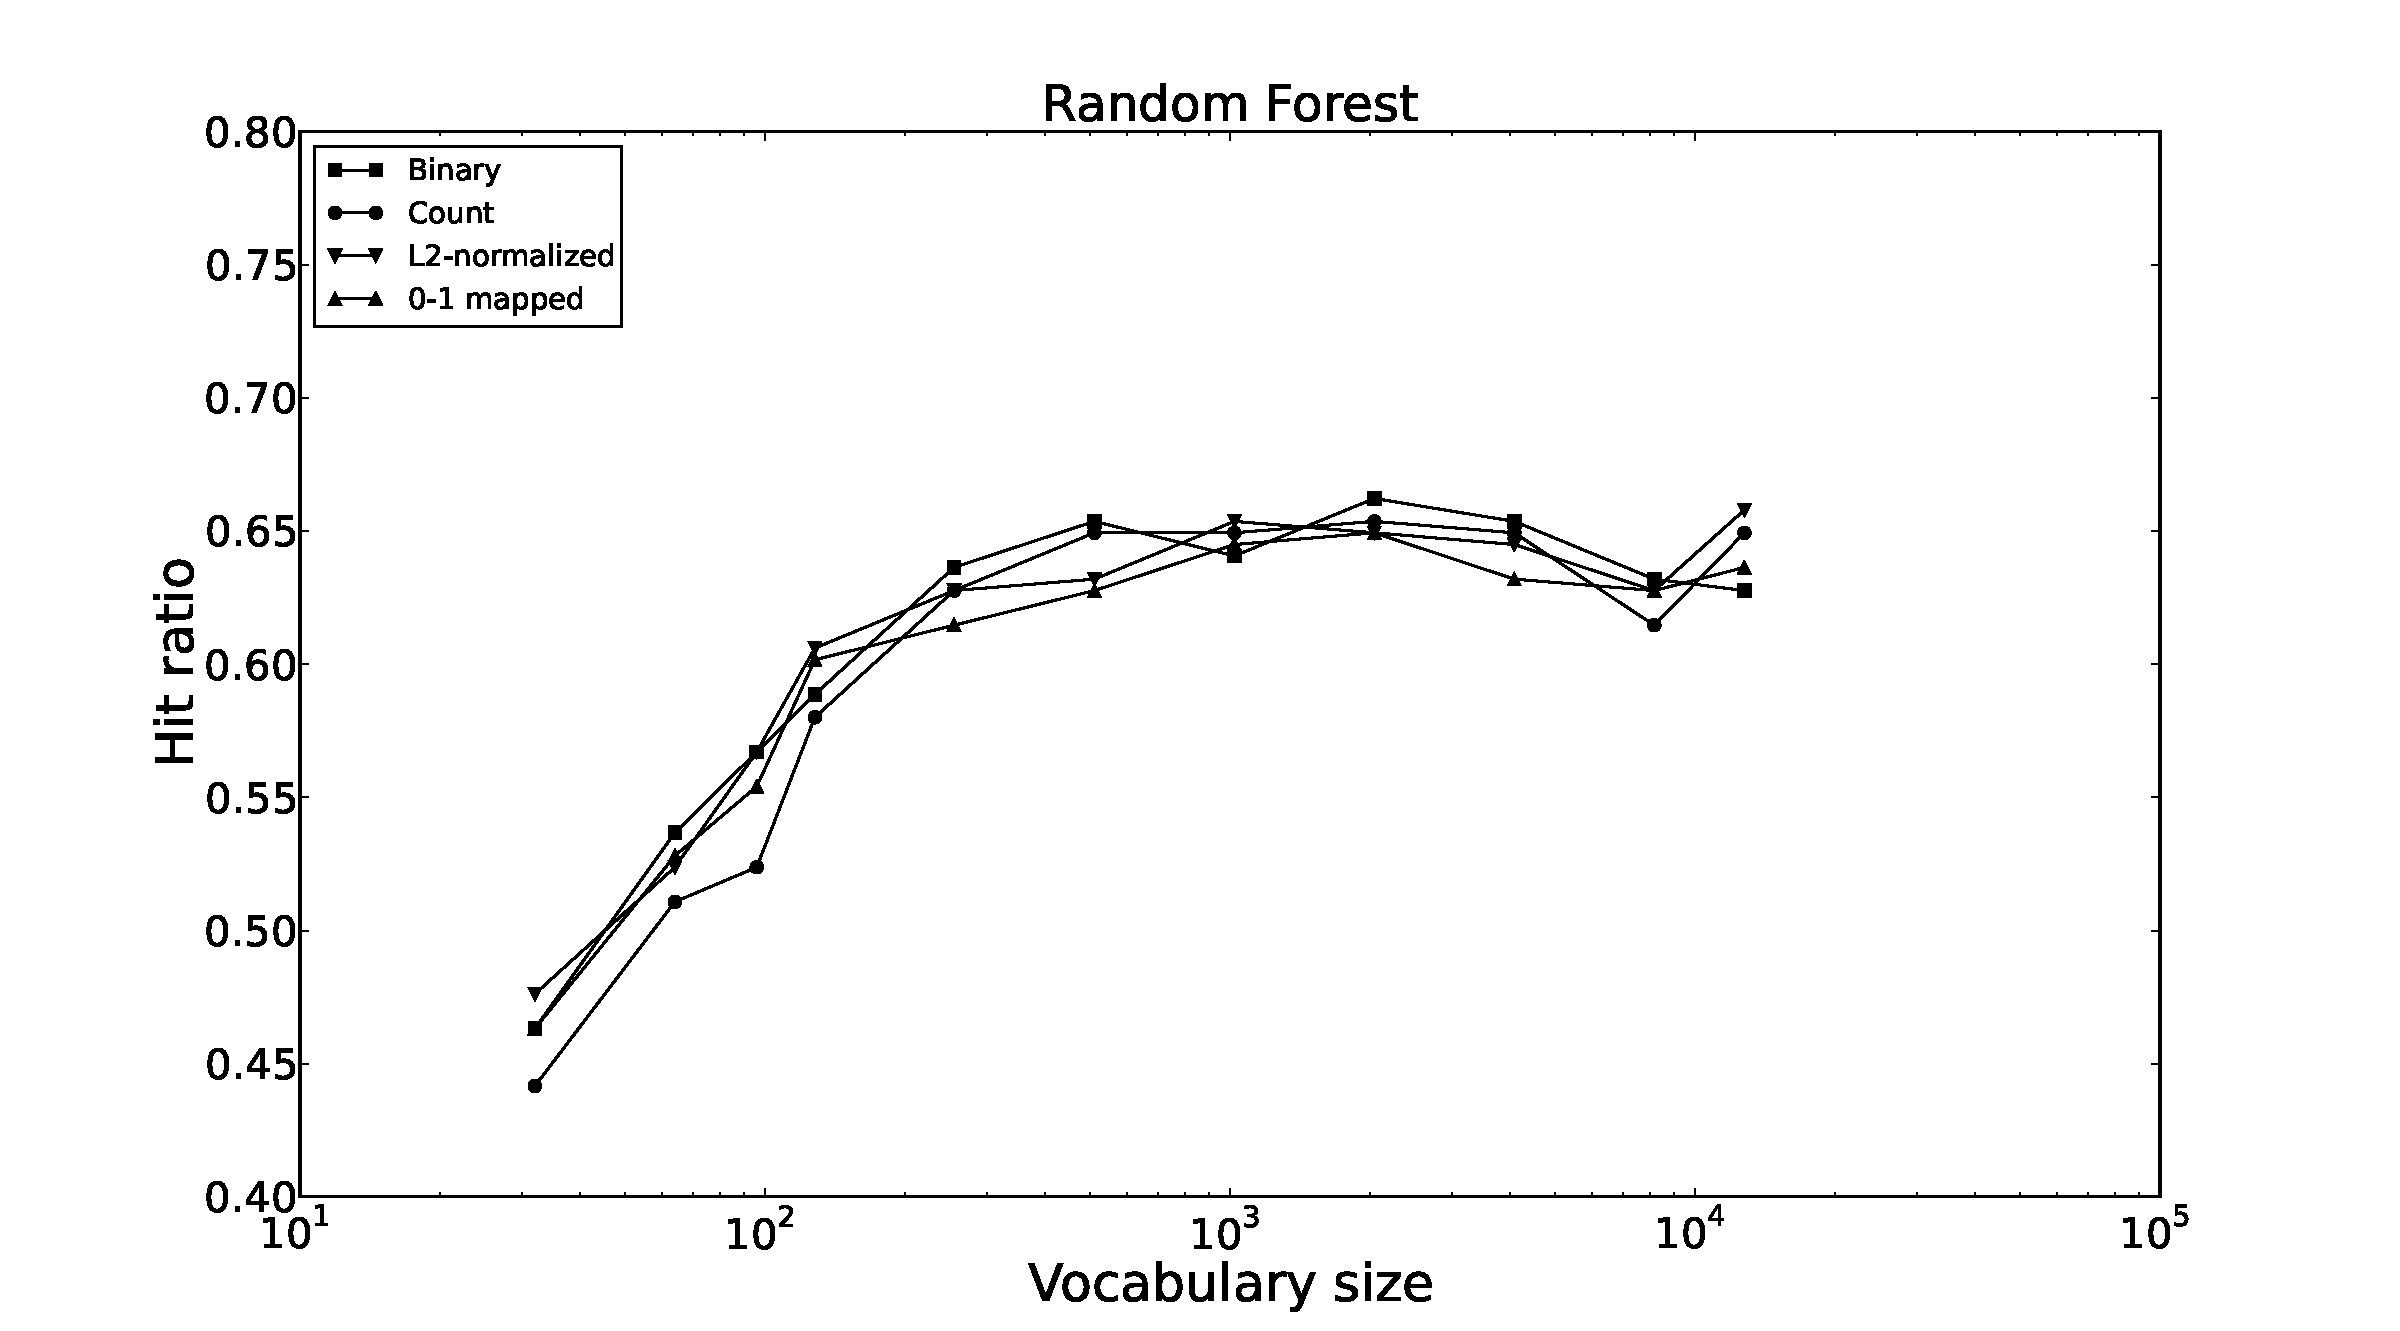
\includegraphics[width=\textwidth]{img/Random-Forest-hitrate-eps-converted-to.pdf}
		\caption{Hit ratio of Random Forest classifier with varying vocabulary size.}
		\label{fig:hitratio-rf}
	\end{subfigure}
	~
	\begin{subfigure}[b]{\figwidth}
		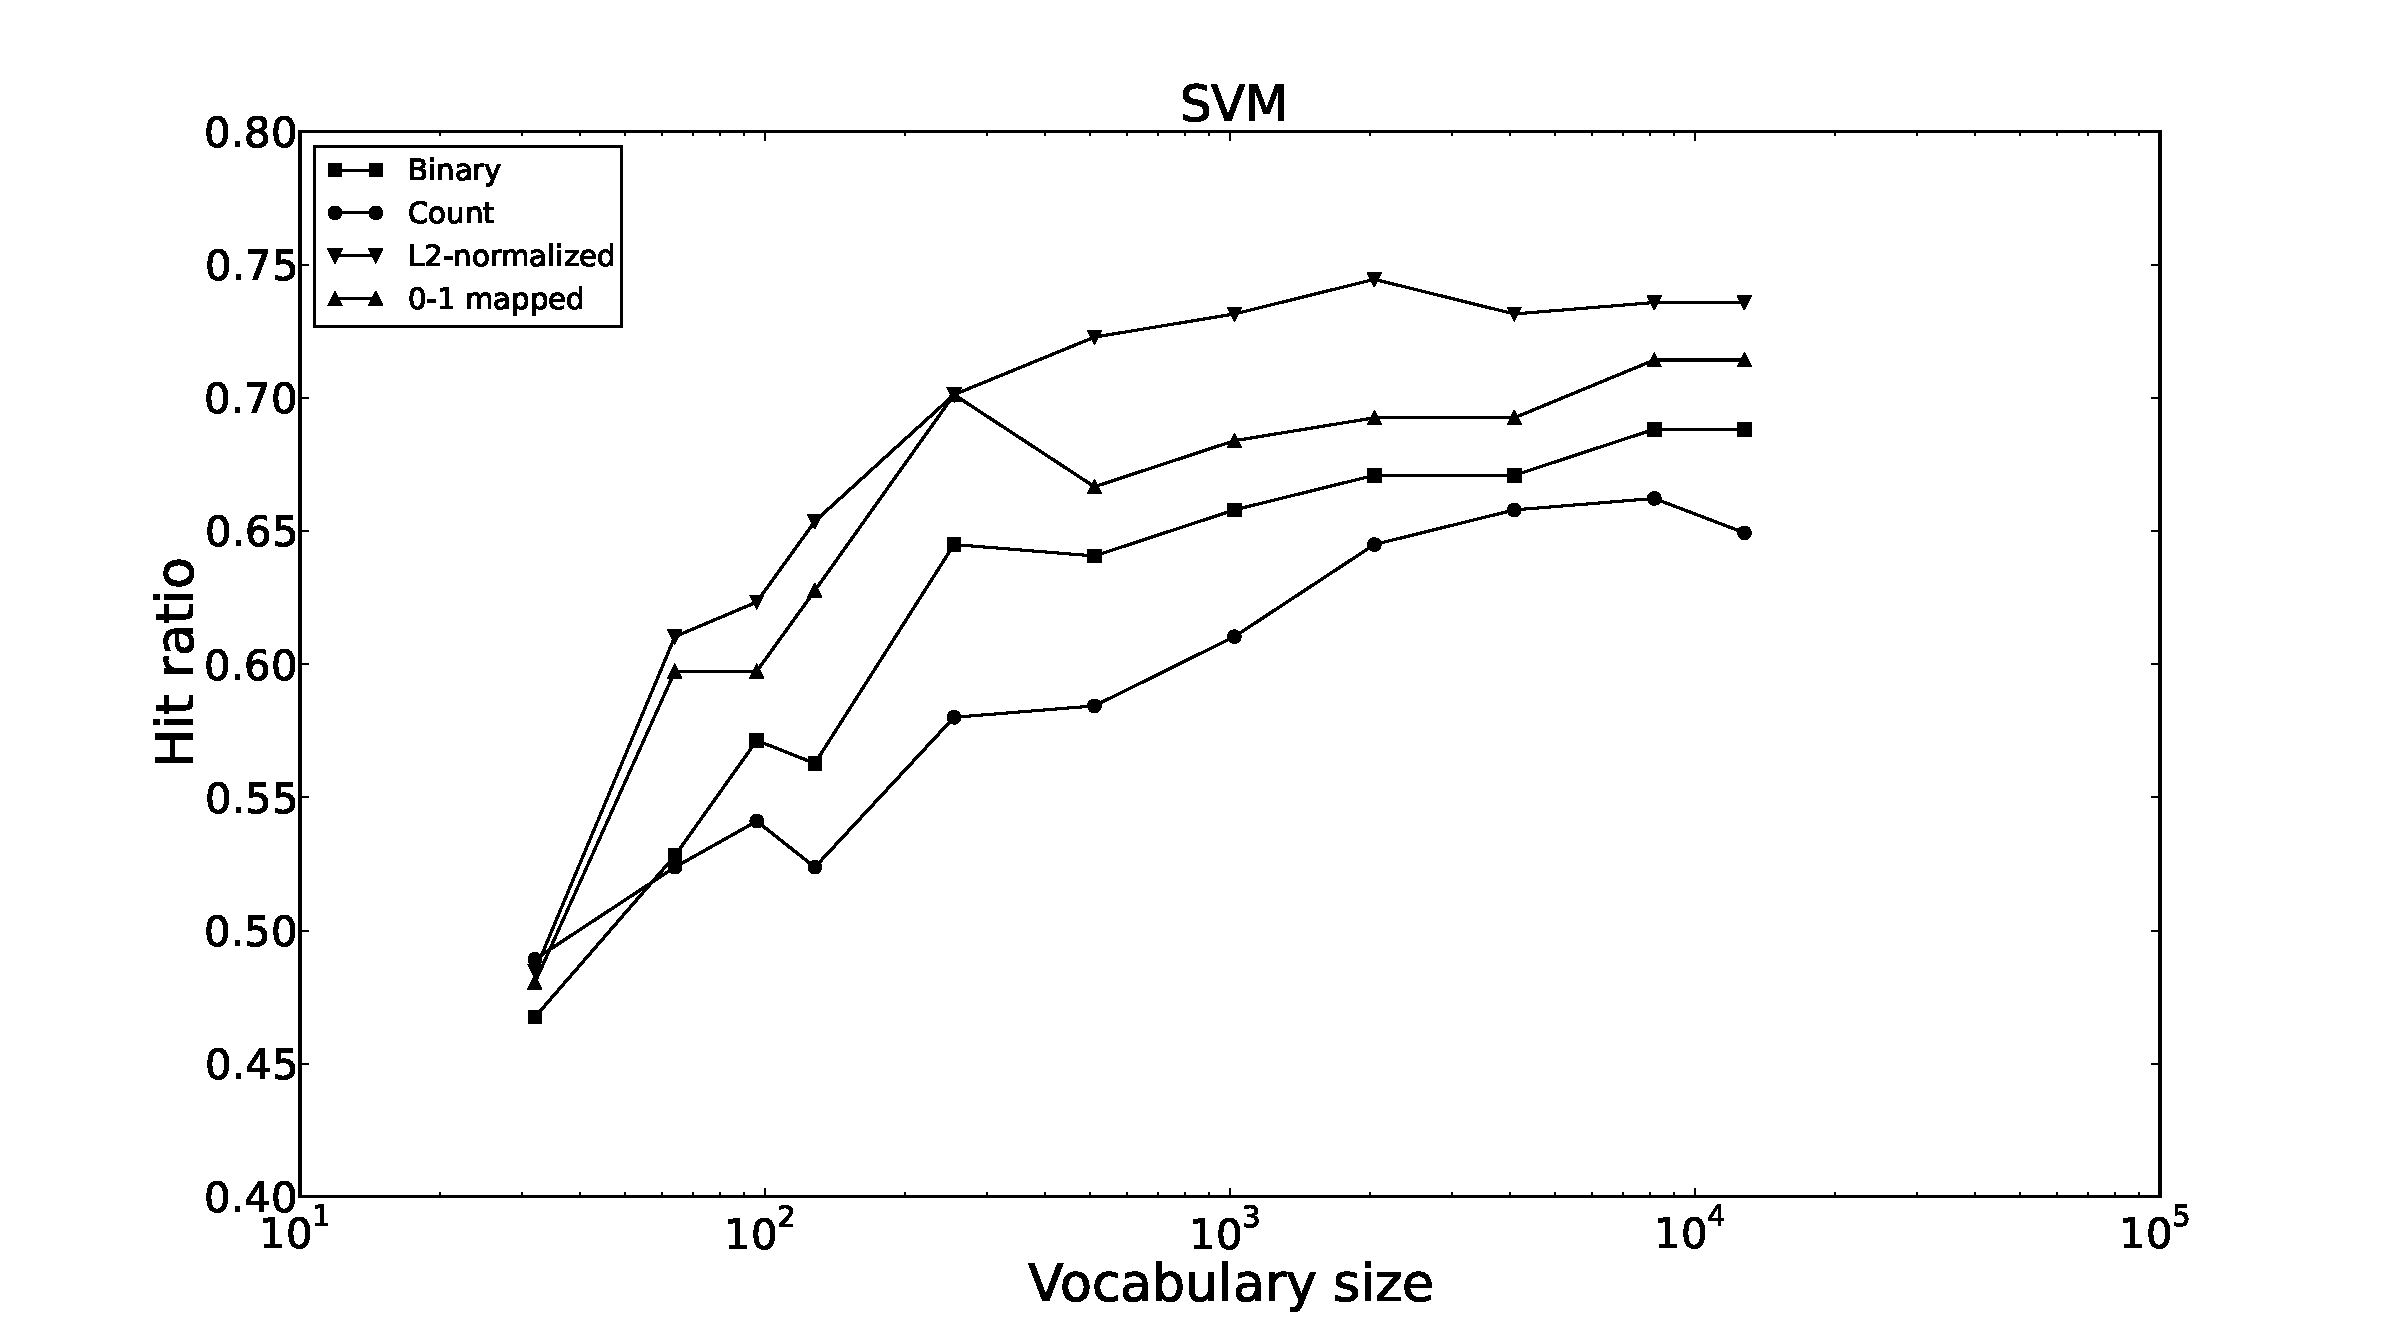
\includegraphics[width=\textwidth]{img/SVM-hitrate-eps-converted-to.pdf}
		\caption{Hit ratio of SVM classifier with varying vocabulary size.}
		\label{fig:hitratio-svm}
	\end{subfigure}
	\\
	\begin{subfigure}[b]{\figwidth}
		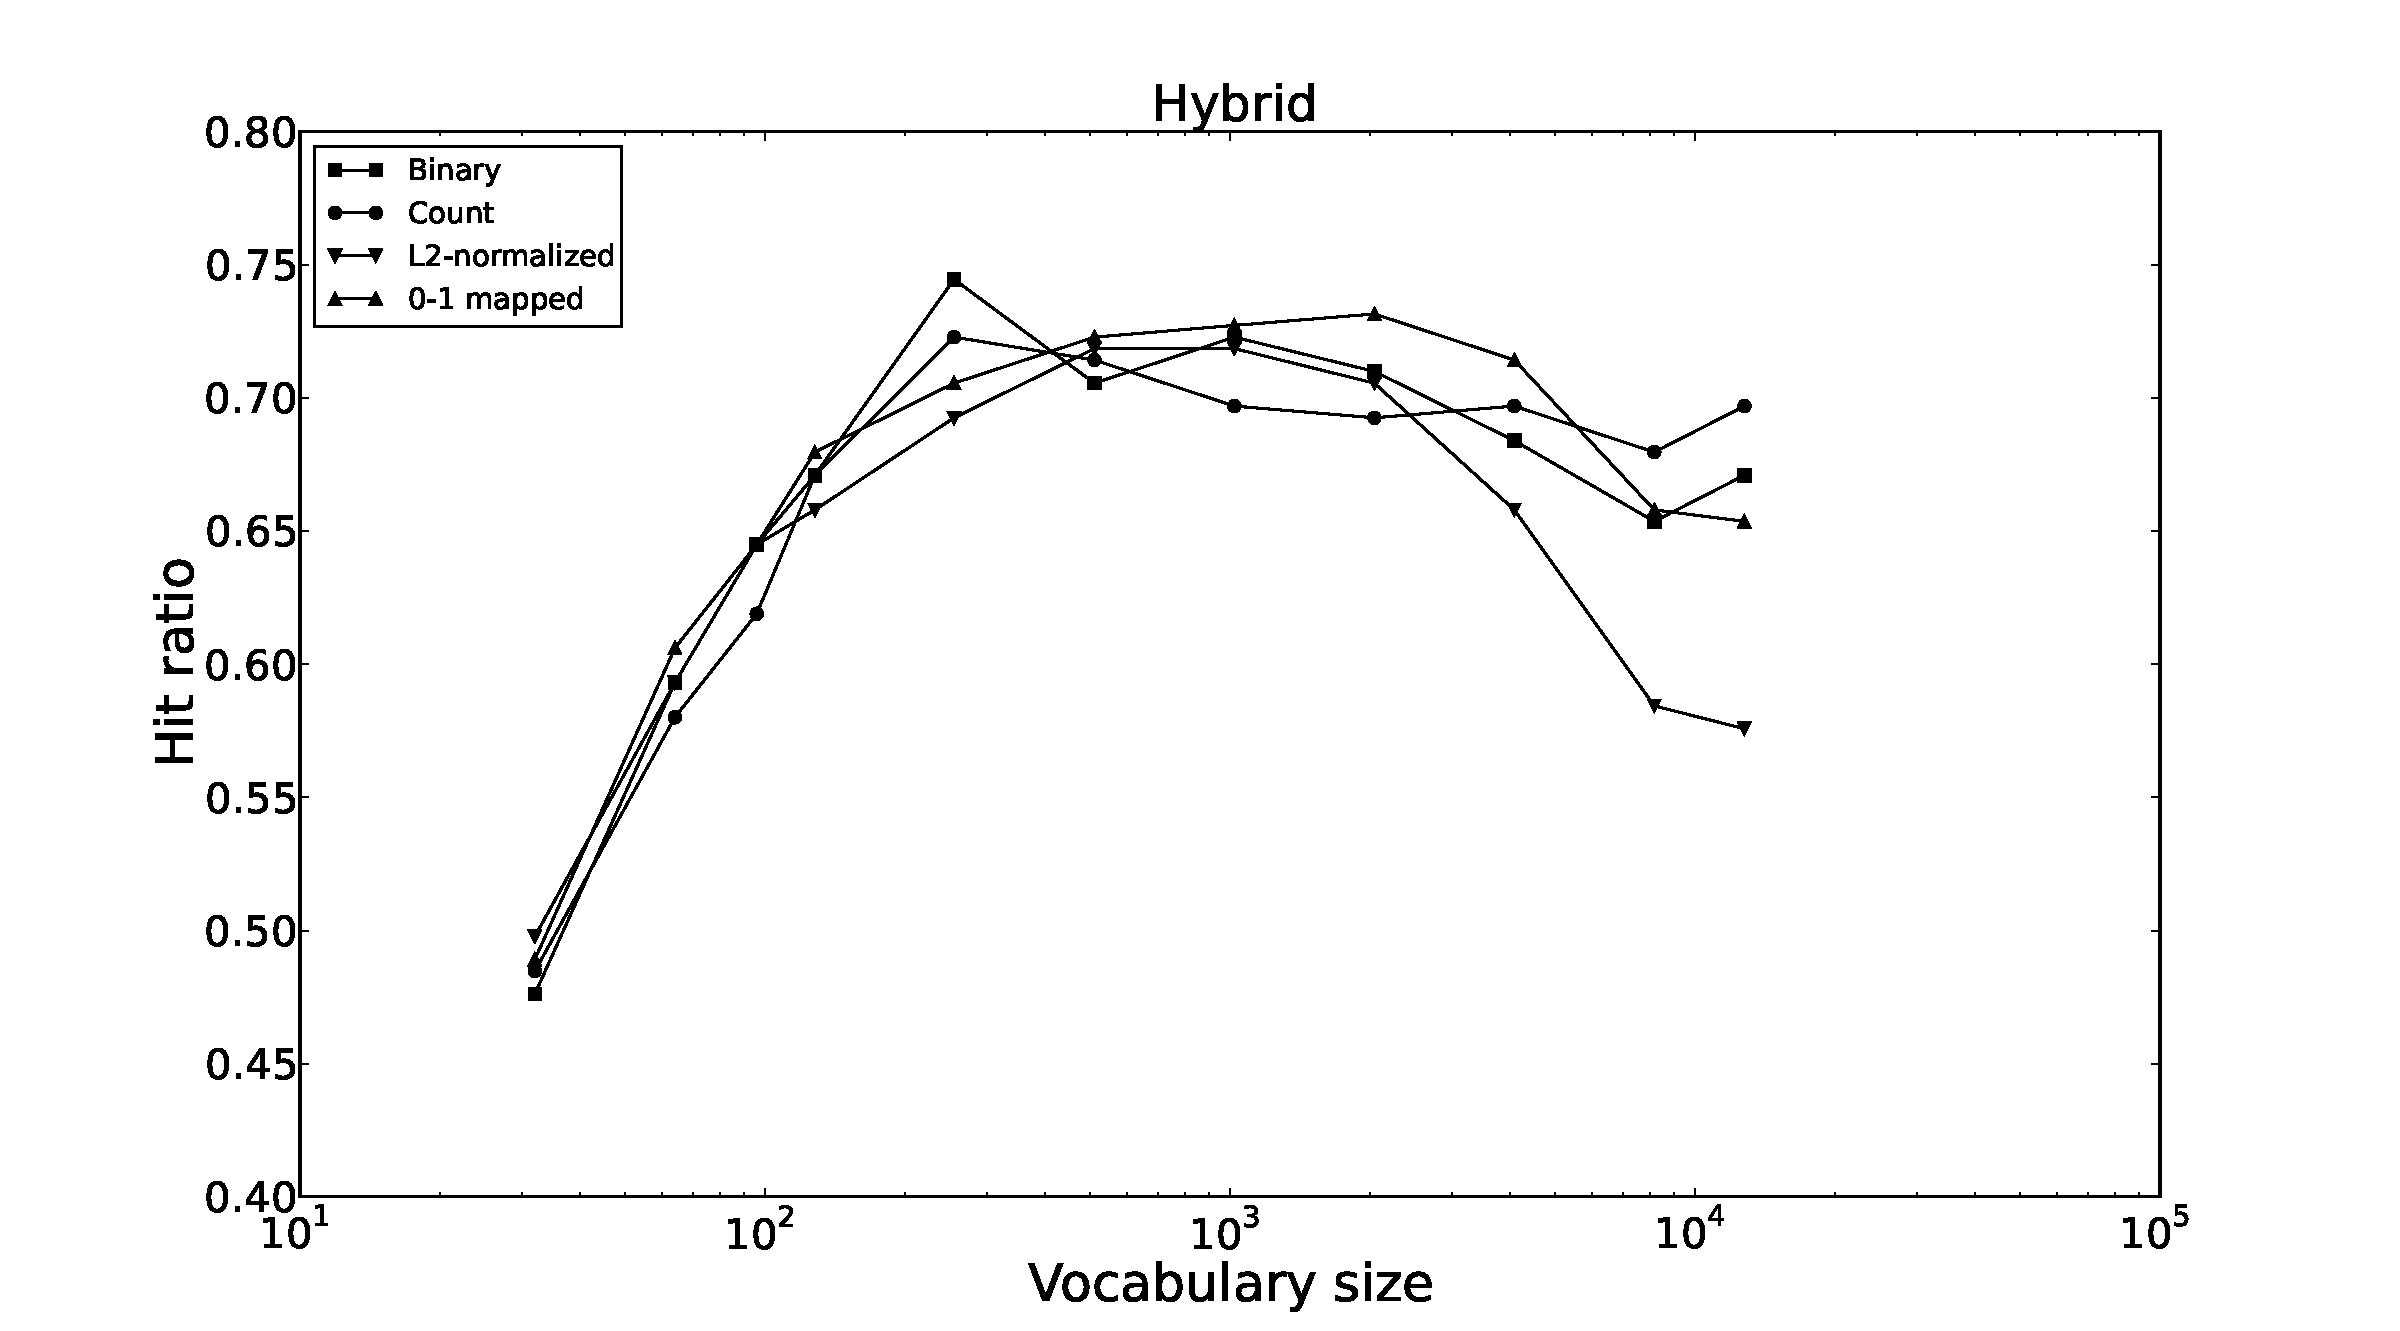
\includegraphics[width=\textwidth]{img/Hybrid-hitrate-eps-converted-to.pdf}
		\caption{Hit ratio of Hybrid classifier with varying vocabulary size.}
		\label{fig:hitratio-hybrid}
	\end{subfigure}
	\caption{Hit ratio vs vocabulary size}
	\label{fig:hitratio}
\end{figure}


\onecolumn
\renewcommand{\figwidth}{0.43\textwidth}
\begin{figure}[H]
	\centering
	\begin{subfigure}[b]{\figwidth}
		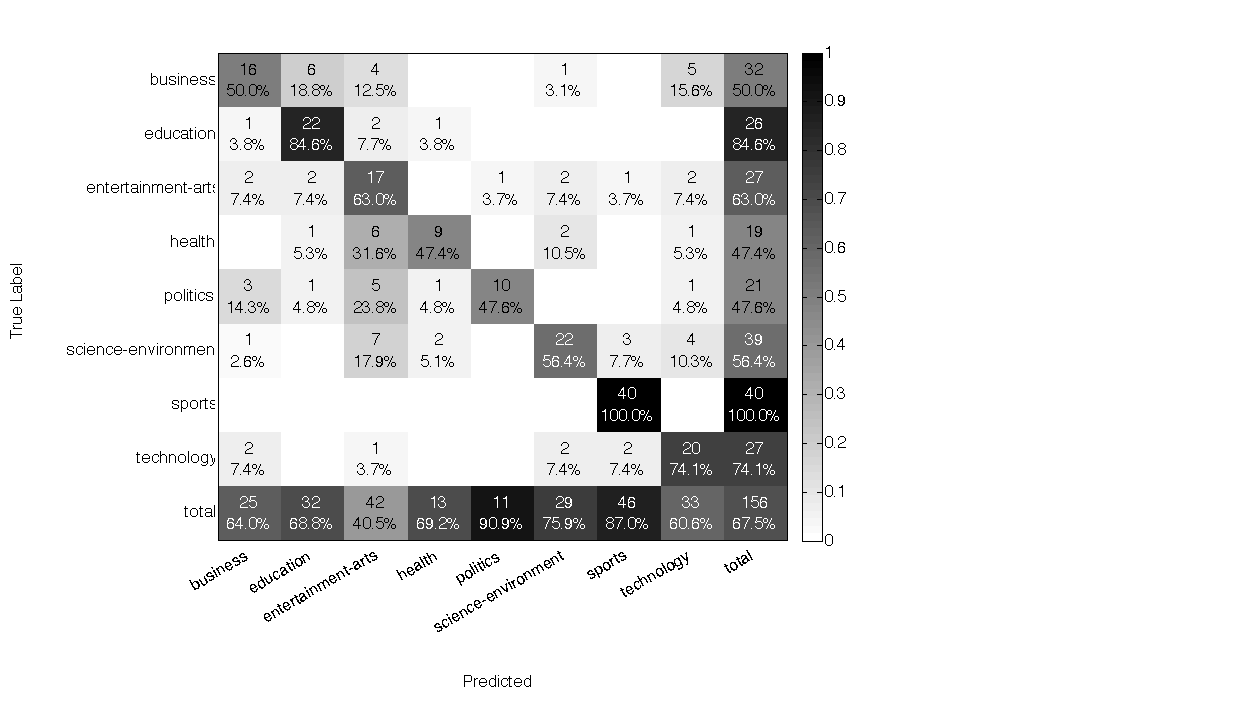
\includegraphics[width=\textwidth,trim=0 0 350 0, clip]{img/Bernou_percentile_5_count.png}
		\caption{Confusion matrix of Bernoulli.}
		\label{fig:confmat-be}
	\end{subfigure}
	~
	\begin{subfigure}[b]{\figwidth}
		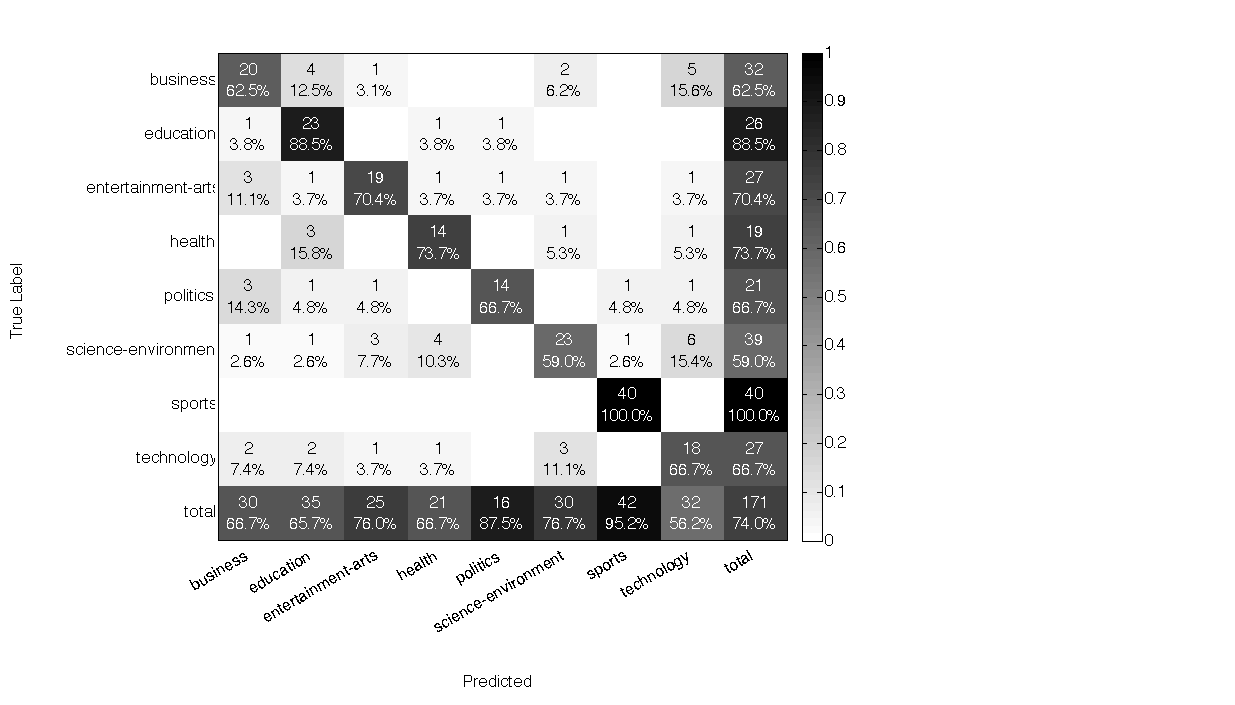
\includegraphics[width=\textwidth,trim=0 0 350 0, clip]{img/Multinomial_percentile_5_count.png}
		\caption{Confusion matrix of Multinomial.}
		\label{fig:confmat-mn}
	\end{subfigure}
	\\
	\begin{subfigure}[b]{\figwidth}
		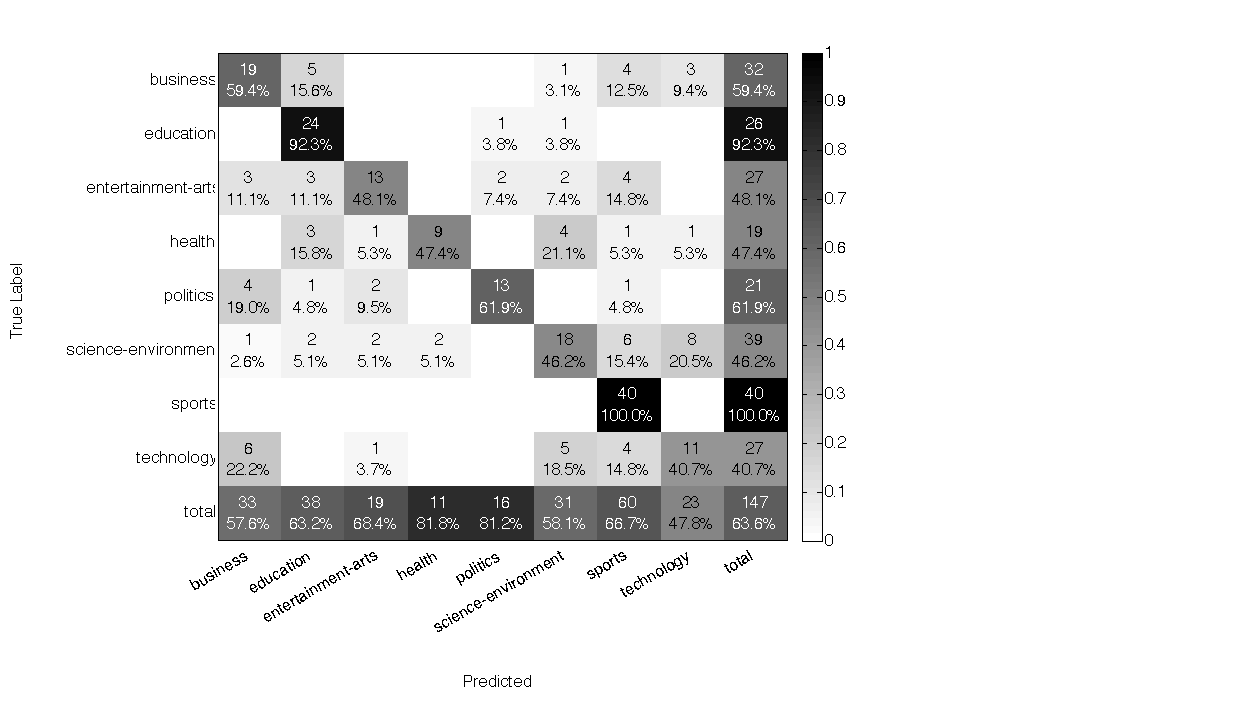
\includegraphics[width=\textwidth,trim=0 0 350 0, clip]{img/RandomForest_percentile_5_count.png}
		\caption{Confusion matrix of Random Forest.}
		\label{fig:confmat-rf}
	\end{subfigure}
	~
	\begin{subfigure}[b]{\figwidth}
		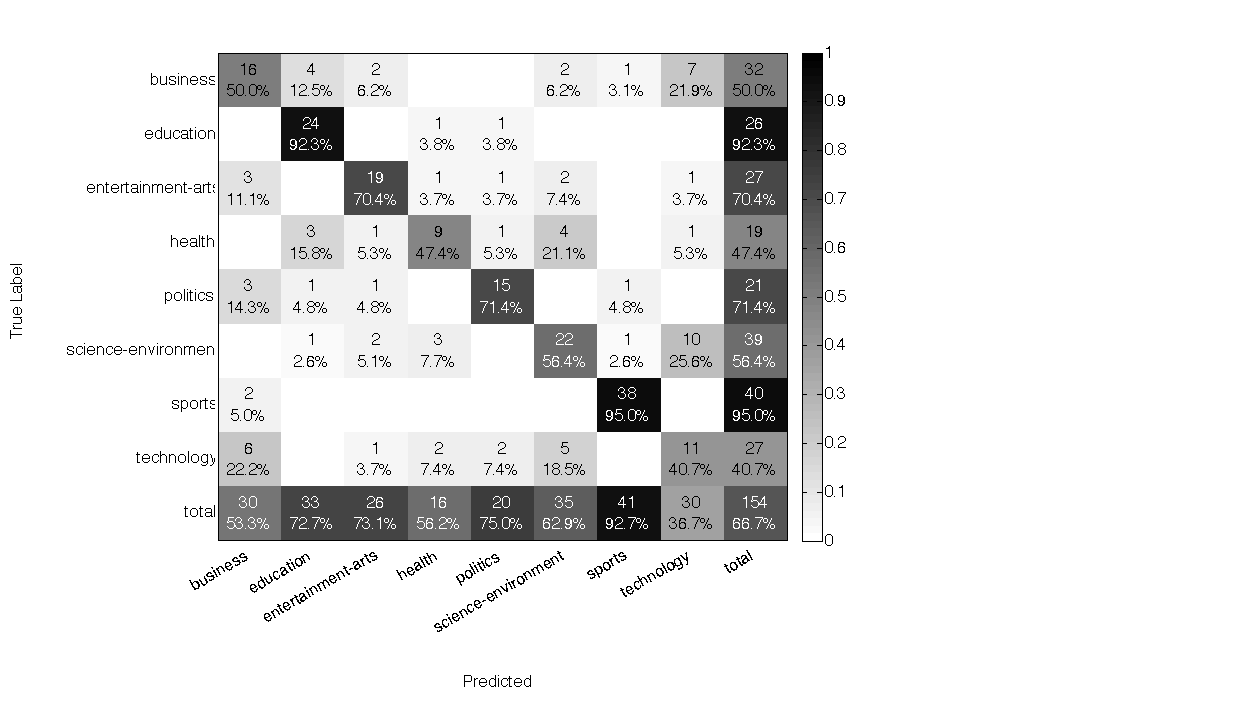
\includegraphics[width=\textwidth,trim=0 0 350 0, clip]{img/SVM_percentile_5_count.png}
		\caption{Confusion matrix of SVM.}
		\label{fig:confmat-svm}
	\end{subfigure}
	\\
	\begin{subfigure}[b]{\figwidth}
		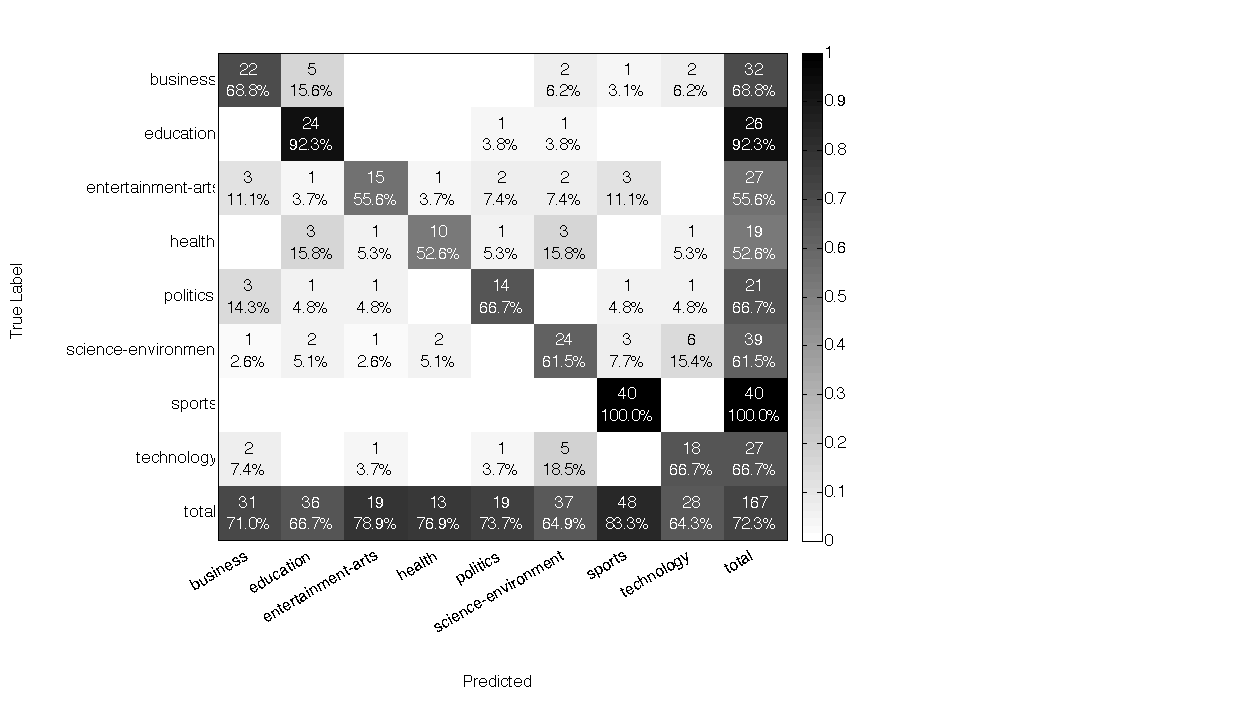
\includegraphics[width=\textwidth,trim=0 0 350 0, clip]{img/hybrid_percentile_5_count.png}
		\caption{Confusion matrix of Hybrid.}
		\label{fig:confmat-hybrid}
	\end{subfigure}
	\caption{Confusion matrices for the different classifiers. A total of 231 articles were tested. A vocabulary size of 511 words and the data type \emph{"Mapped value form 0 to 1"} were used.}
	\label{fig:confmat}
\end{figure}

\onecolumn
\setlength\figureheight{0.25\linewidth}
\setlength\figurewidth{0.35\linewidth}
\begin{figure}[H]
	\centering
	\begin{subfigure}[b]{\figwidth}
		\tikzstyle{every node}=[font=\scriptsize]
		% This file was created by matlab2tikz v0.4.3.
% Copyright (c) 2008--2013, Nico Schlömer <nico.schloemer@gmail.com>
% All rights reserved.
% 
% The latest updates can be retrieved from
%   http://www.mathworks.com/matlabcentral/fileexchange/22022-matlab2tikz
% where you can also make suggestions and rate matlab2tikz.
% 
\begin{tikzpicture}

\begin{axis}[%
width=\figurewidth,
height=\figureheight,
scale only axis,
xmin=0,
xmax=503,
xlabel={Number of articles in training data},
ymin=0.5,
ymax=0.8,
ylabel={Hit ratio},
title={Bernoulli}
]
\addplot [
color=black,
solid,
mark=square,
mark options={solid},
forget plot
]
table[row sep=crcr]{
6 0.5325\\
11 0.6147\\
16 0.632\\
21 0.6407\\
41 0.6537\\
81 0.6753\\
161 0.6797\\
322 0.671\\
503 0.671\\
};
\addplot [
color=black,
solid,
mark=o,
mark options={solid},
forget plot
]
table[row sep=crcr]{
6 0.5325\\
11 0.6147\\
16 0.632\\
21 0.6407\\
41 0.6537\\
81 0.6753\\
161 0.6797\\
322 0.671\\
503 0.671\\
};
\addplot [
color=black,
solid,
mark=triangle,
mark options={solid,,rotate=180},
forget plot
]
table[row sep=crcr]{
6 0.5325\\
11 0.6147\\
16 0.632\\
21 0.6407\\
41 0.6537\\
81 0.6753\\
161 0.6797\\
322 0.671\\
503 0.671\\
};
\addplot [
color=black,
solid,
mark=triangle,
mark options={solid},
forget plot
]
table[row sep=crcr]{
6 0.5325\\
11 0.6147\\
16 0.632\\
21 0.6407\\
41 0.6537\\
81 0.6753\\
161 0.6797\\
322 0.671\\
503 0.671\\
};
\end{axis}
\end{tikzpicture}%
		\caption{Hit ratio of Bernoulli classifier with varying number of articles in training data. All values greater than zero are mapped to one, hence the different data types result in the same accuracy.}
		\label{fig:hitratio-data-nb}
	\end{subfigure}
	~
	\begin{subfigure}[b]{\figwidth}
		\tikzstyle{every node}=[font=\scriptsize]
		% This file was created by matlab2tikz v0.4.3.
% Copyright (c) 2008--2013, Nico Schlömer <nico.schloemer@gmail.com>
% All rights reserved.
% 
% The latest updates can be retrieved from
%   http://www.mathworks.com/matlabcentral/fileexchange/22022-matlab2tikz
% where you can also make suggestions and rate matlab2tikz.
% 
\begin{tikzpicture}

\begin{axis}[%
width=\figurewidth,
height=\figureheight,
scale only axis,
xmin=0,
xmax=503,
xlabel={Number of articles in training data},
ymin=0.5,
ymax=0.8,
ylabel={Hit ratio},
title={Multinomial}
]
\addplot [
color=black,
solid,
mark=square,
mark options={solid},
forget plot
]
table[row sep=crcr]{
6 0.6667\\
11 0.7186\\
16 0.7316\\
21 0.7316\\
41 0.7446\\
81 0.7532\\
161 0.7706\\
322 0.7316\\
503 0.7229\\
};
\addplot [
color=black,
solid,
mark=o,
mark options={solid},
forget plot
]
table[row sep=crcr]{
6 0.6883\\
11 0.7013\\
16 0.7186\\
21 0.7273\\
41 0.7403\\
81 0.7186\\
161 0.7489\\
322 0.7359\\
503 0.7446\\
};
\addplot [
color=black,
solid,
mark=triangle,
mark options={solid,,rotate=180},
forget plot
]
table[row sep=crcr]{
6 0.5844\\
11 0.6407\\
16 0.6753\\
21 0.684\\
41 0.7013\\
81 0.6883\\
161 0.6883\\
322 0.6883\\
503 0.6926\\
};
\addplot [
color=black,
solid,
mark=triangle,
mark options={solid},
forget plot
]
table[row sep=crcr]{
6 0.645\\
11 0.6883\\
16 0.7359\\
21 0.7316\\
41 0.7489\\
81 0.7446\\
161 0.7359\\
322 0.7186\\
503 0.7273\\
};
\end{axis}
\end{tikzpicture}%
		\caption{Hit ratio of Multinomial classifier with varying number of articles in training data.\\\ \\\ }
		\label{fig:hitratio-data-mn}
	\end{subfigure}
	\\
	\begin{subfigure}[b]{\figwidth}
		\tikzstyle{every node}=[font=\scriptsize]
		% This file was created by matlab2tikz v0.4.3.
% Copyright (c) 2008--2013, Nico Schlömer <nico.schloemer@gmail.com>
% All rights reserved.
% 
% The latest updates can be retrieved from
%   http://www.mathworks.com/matlabcentral/fileexchange/22022-matlab2tikz
% where you can also make suggestions and rate matlab2tikz.
% 
\begin{tikzpicture}

\begin{axis}[%
width=\figurewidth,
height=\figureheight,
scale only axis,
xmin=0,
xmax=503,
xlabel={Number of articles in training data},
ymin=0.5,
ymax=0.8,
ylabel={Hit ratio},
title={Random Forest}
]
\addplot [
color=black,
solid,
mark=square,
mark options={solid},
forget plot
]
table[row sep=crcr]{
6 0.5281\\
11 0.5714\\
16 0.6017\\
21 0.619\\
41 0.6623\\
81 0.658\\
161 0.684\\
322 0.645\\
503 0.6494\\
};
\addplot [
color=black,
solid,
mark=o,
mark options={solid},
forget plot
]
table[row sep=crcr]{
6 0.5541\\
11 0.5887\\
16 0.6147\\
21 0.619\\
41 0.6623\\
81 0.6623\\
161 0.6537\\
322 0.6537\\
503 0.6364\\
};
\addplot [
color=black,
solid,
mark=triangle,
mark options={solid,,rotate=180},
forget plot
]
table[row sep=crcr]{
6 0.5368\\
11 0.5974\\
16 0.6234\\
21 0.6407\\
41 0.632\\
81 0.645\\
161 0.6364\\
322 0.6407\\
503 0.6277\\
};
\addplot [
color=black,
solid,
mark=triangle,
mark options={solid},
forget plot
]
table[row sep=crcr]{
6 0.5238\\
11 0.5931\\
16 0.6277\\
21 0.6234\\
41 0.6234\\
81 0.6537\\
161 0.645\\
322 0.6407\\
503 0.6407\\
};
\end{axis}
\end{tikzpicture}%
		\caption{Hit ratio of Random Forest classifier with varying number of articles in training data.}
		\label{fig:hitratio-data-rf}
	\end{subfigure}
	~
	\begin{subfigure}[b]{\figwidth}
		\tikzstyle{every node}=[font=\scriptsize]
		% This file was created by matlab2tikz v0.4.3.
% Copyright (c) 2008--2013, Nico Schlömer <nico.schloemer@gmail.com>
% All rights reserved.
% 
% The latest updates can be retrieved from
%   http://www.mathworks.com/matlabcentral/fileexchange/22022-matlab2tikz
% where you can also make suggestions and rate matlab2tikz.
% 
\begin{tikzpicture}

\begin{axis}[%
width=\figurewidth,
height=\figureheight,
scale only axis,
xmin=0,
xmax=503,
xlabel={Number of articles in training data},
ymin=0.5,
ymax=0.8,
ylabel={Hit ratio},
title={SVM}
]
\addplot [
color=black,
solid,
mark=square,
mark options={solid},
forget plot
]
table[row sep=crcr]{
6 0.5108\\
11 0.5238\\
16 0.6017\\
21 0.5801\\
41 0.6407\\
81 0.6667\\
161 0.6537\\
322 0.6407\\
503 0.6407\\
};
\addplot [
color=black,
solid,
mark=o,
mark options={solid},
forget plot
]
table[row sep=crcr]{
6 0.5065\\
11 0.5238\\
16 0.5887\\
21 0.6017\\
41 0.6234\\
81 0.5844\\
161 0.5584\\
322 0.5887\\
503 0.5758\\
};
\addplot [
color=black,
solid,
mark=triangle,
mark options={solid,,rotate=180},
forget plot
]
table[row sep=crcr]{
6 0.6407\\
11 0.6623\\
16 0.7273\\
21 0.7013\\
41 0.7186\\
81 0.7489\\
161 0.7532\\
322 0.7359\\
503 0.7273\\
};
\addplot [
color=black,
solid,
mark=triangle,
mark options={solid},
forget plot
]
table[row sep=crcr]{
6 0.6104\\
11 0.5974\\
16 0.658\\
21 0.6537\\
41 0.6797\\
81 0.671\\
161 0.6926\\
322 0.6667\\
503 0.6537\\
};
\end{axis}
\end{tikzpicture}%
		\caption{Hit ratio of SVM classifier with varying number of articles in training data.}
		\label{fig:hitratio-data-svm}
	\end{subfigure}
	\\
	\begin{subfigure}[b]{\figwidth}
		\tikzstyle{every node}=[font=\scriptsize]
		% This file was created by matlab2tikz v0.4.3.
% Copyright (c) 2008--2013, Nico Schlömer <nico.schloemer@gmail.com>
% All rights reserved.
% 
% The latest updates can be retrieved from
%   http://www.mathworks.com/matlabcentral/fileexchange/22022-matlab2tikz
% where you can also make suggestions and rate matlab2tikz.
% 
\begin{tikzpicture}

\begin{axis}[%
width=\figurewidth,
height=\figureheight,
scale only axis,
xmin=0,
xmax=503,
xlabel={Number of articles in training data},
ymin=0.5,
ymax=0.8,
ylabel={Hit ratio},
title={Hybrid},
legend style={at={(1.03,1)},anchor=north west,draw=black,fill=white,legend cell align=left}
]
\addplot [
color=black,
solid,
mark=square,
mark options={solid}
]
table[row sep=crcr]{
6 0.6234\\
11 0.6494\\
16 0.6883\\
21 0.7013\\
41 0.7056\\
81 0.7186\\
161 0.7273\\
322 0.7056\\
503 0.7013\\
};
\addlegendentry{Binary};

\addplot [
color=black,
solid,
mark=o,
mark options={solid}
]
table[row sep=crcr]{
6 0.6537\\
11 0.658\\
16 0.697\\
21 0.6926\\
41 0.7143\\
81 0.6883\\
161 0.71\\
322 0.7056\\
503 0.7273\\
};
\addlegendentry{Count};

\addplot [
color=black,
solid,
mark=triangle,
mark options={solid,,rotate=180}
]
table[row sep=crcr]{
6 0.5931\\
11 0.645\\
16 0.6926\\
21 0.697\\
41 0.7143\\
81 0.7229\\
161 0.7186\\
322 0.7186\\
503 0.7229\\
};
\addlegendentry{L2-normalized};

\addplot [
color=black,
solid,
mark=triangle,
mark options={solid}
]
table[row sep=crcr]{
6 0.619\\
11 0.6623\\
16 0.7143\\
21 0.7056\\
41 0.7143\\
81 0.7143\\
161 0.7316\\
322 0.7186\\
503 0.7273\\
};
\addlegendentry{0-1 mapped};

\end{axis}
\end{tikzpicture}%
		\caption{Hit ratio of Hybrid classifier with varying number of articles in training data.}
		\label{fig:hitratio-data-hybrid}
	\end{subfigure}
	\caption{Hit ratio as a function of number of articles in training data for different classifiers and data types at a constant vocabulary size of 500 features after $\chi^2$ selection.}
	\label{fig:hitratio-data}
\end{figure}
\twocolumn

\section{Related work}
\subsection{\nb\ Classifier}
	Naïve Bayes models are widely used because of it's simplicity and efficiency. A. McCallum and K. Nigam compares the two most common models, the multi-variate Bernoulli and the multinomial model, in the realm of document classification. They are explained in detailed both theoretically and empirically and in general the multinomial model outperforms the Bernoulli model \cite{McCallum98acomparison}.
\subsection{\rf\ Classifier}
Random Forest is a decision tree based classification model. It has been used to classify web documents by keywords, where it for five and seven topics performed better than ,e.g., Naïve Bayes and MLP. In the paper by Kopriska \emph{et al.} they use Random Forest for classifying e-mails. Random Forest was able to out perform other methods, such as DT, SVM and NB. \cite{keywords}\cite{email}
\subsection{\svm\ Classifier}
\subsection{Support Vector Machine Classifier}
Support vector machine classifiers performs well on data that is linearly separable and is guaranteed to find the optimal hyperplane that separates the data. They can however only separate data into two classes, but if combined they are able to perform multi-class classification. A simple approach is to use $k$ SVMs to solve a $k$-class classification problem. The SVMs may also be combined in a more sophisticated fashion, so that less than $k$ SVMs can be used. Both methods are investigated in \cite{Mayoras99SVM}.

\section{Conclusions \& Future work}
%%%%%%%%%%%%%%%%%%%% DRAFT %%%%%%%%%%%%%%
\ifnum\printdraft>0
	\begin{itemize}
		%\item Fuzzy match example for improvement or testing.
		%\item Term Frequency - Inverse Document Frequency (TF-IDF) is an interesting way of mapping the data so that terms that are unique for certain classes are emphasized.
		\item ANOVA F-value
		\item Use document characteristics as features such as average word length, number of tokens representing digits etc.
	\end{itemize}
\else
\begin{center}
	\textbf{--- DRAFT PARTS ---}
\end{center}
\fi
%%%%%%%%%%%%%%%%%%%% END DRAFT %%%%%%%%%%
\mn\ \nb\ proved to be the most suitable classifier for the task of classifying news articles of eight different classes, since it obtained the highest hit ratio and had a good overall performance for different datatypes.
\\\\
\svm\ proved to be the classifier that is most sensitive of the data type. Figures \ref{fig:hitratio} and \ref{fig:hitratio-data} show that the performance is poor for the data type count and that the performance is best for the $L_2$-normalized data.
\\\\
It would be of interest as future work to do an investigation of how the \rf\ classifier behaves if the data is evenly balanced between the classes. For further reading in the field of very imbalanced data, see \cite{Chen}.
\\\\
Future work would also include analyzing other pruning techniques, e.g. TF-IDF which emphasizes words that are unique for a document and suppress the value of common words among all documents. 


\bibliographystyle{plain}
\bibliography{bibliography}
\nocite{*}

% \begin{thebibliography}{99}
% 	\bibitem{nb_thoery}\href{http://www.aaai.org/Papers/FLAIRS/2004/Flairs04-097.pdf}{Harry Zhang, The Optimality of Naive Bayes, AA, 2004}
% 	\bibitem{nb_comparison}\href{http://citeseerx.ist.psu.edu/viewdoc/download?doi=10.1.1.65.9324&rep=rep1&type=pdf}{McCallum and K. Nigam. “A Comparison of Event Models for Naive Bayes Text Classification” }
% \end{thebibliography}

\end{document}
